\documentclass[11pt,aspectratio=169,usepdftitle=false]{beamer}

\usepackage[T1]{fontenc}
\usepackage{lmodern}
\usepackage{amsmath,amssymb,mathtools}
\usepackage{booktabs}
\usepackage{microtype}
\usepackage{appendixnumberbeamer}
\usepackage{tikz}
\usetikzlibrary{arrows.meta,calc,decorations.pathreplacing,positioning,shapes.geometric}

\definecolor{AuburnNavy}{HTML}{03244D}
\definecolor{AuburnOrange}{HTML}{DD550C}
\definecolor{DeepTeal}{HTML}{007D8A}
\definecolor{LeafGreen}{HTML}{2E7D32}
\definecolor{WarmGold}{HTML}{F2B134}
\definecolor{Ink}{HTML}{17212B}
\definecolor{Slate}{HTML}{5E6B78}
\definecolor{Mist}{HTML}{EEF3F7}
\definecolor{Cream}{HTML}{FFF9F2}
\definecolor{SoftRed}{HTML}{B3261E}

% -----------------------------------------------------------------------------
% Mother-deck switches.  The canonical archive keeps every switch true.
% Turn selected switches off for a shorter venue-specific talk.
% -----------------------------------------------------------------------------
\newif\ifshowoddslack
\newif\ifshowcalibration
\newif\ifshowbarriers
\newif\ifshowfrontier
\newif\ifshowverification
\showoddslacktrue
\showcalibrationtrue
\showbarrierstrue
\showfrontiertrue
\showverificationtrue

% -----------------------------------------------------------------------------
% Metadata: plain-text PDF strings are set explicitly because Beamer's visual
% title uses TeX line breaks and mathematical notation.
% -----------------------------------------------------------------------------
\title{How Much Area Does a Circle Force?}
\subtitle{Gromov's filling-area conjecture through distance profiles and Fourier modes}
\author{Le Chen}
\institute{Auburn University\\[0.15em]\scriptsize Joint work with Xiaolong Li and Yimin Zhong}
\date{Mother deck --- September 2026}
\hypersetup{
pdftitle={How Much Area Does a Circle Force? Gromov's Filling-Area Conjecture},
pdfauthor={Le Chen; Xiaolong Li; Yimin Zhong},
pdfsubject={Graduate introduction to Gromov's filling-area conjecture and Fourier lower bounds},
pdfkeywords={Gromov filling area conjecture, Riemannian surface, Fourier analysis, calibration, Lean verification},
colorlinks=true,
urlcolor=DeepTeal,
linkcolor=AuburnNavy
}

% -----------------------------------------------------------------------------
% Visual system: Auburn navy/orange with a restrained teal for definitions.
% -----------------------------------------------------------------------------
\usetheme{default}
\usefonttheme{professionalfonts}
\beamertemplatenavigationsymbolsempty
\beamerdefaultoverlayspecification{}
\setbeamersize{text margin left=0.62cm,text margin right=0.62cm}
\setlength{\parskip}{0.28em}

\setbeamercolor{normal text}{fg=Ink,bg=white}
\setbeamercolor{structure}{fg=AuburnNavy}
\setbeamercolor{alerted text}{fg=AuburnOrange}
\setbeamercolor{frametitle}{fg=white,bg=AuburnNavy}
\setbeamercolor{title}{fg=white}
\setbeamercolor{subtitle}{fg=Mist}
\setbeamercolor{block title}{fg=white,bg=AuburnNavy}
\setbeamercolor{block body}{fg=Ink,bg=Mist}
\setbeamercolor{block title alerted}{fg=white,bg=AuburnOrange}
\setbeamercolor{block body alerted}{fg=Ink,bg=Cream}
\setbeamercolor{block title example}{fg=white,bg=DeepTeal}
\setbeamercolor{block body example}{fg=Ink,bg=DeepTeal!7}
\setbeamercolor{author in head/foot}{fg=white,bg=AuburnNavy}
\setbeamercolor{date in head/foot}{fg=white,bg=AuburnOrange}

\setbeamerfont{title}{series=\bfseries,size=\fontsize{26}{29}}
\setbeamerfont{subtitle}{size=\large}
\setbeamerfont{frametitle}{series=\bfseries,size=\Large}
\setbeamerfont{block title}{series=\bfseries}
\setbeamerfont{footline}{size=\scriptsize}
\setbeamertemplate{blocks}[rounded][shadow=false]
\setbeamertemplate{itemize item}{\color{AuburnOrange}$\blacktriangleright$}
\setbeamertemplate{itemize subitem}{\color{DeepTeal}$\bullet$}
\setbeamertemplate{enumerate item}{\color{AuburnOrange}\insertenumlabel.}

\setbeamertemplate{frametitle}{%
\nointerlineskip
\begin{beamercolorbox}[wd=\paperwidth,ht=0.72cm,dp=0.20cm,leftskip=0.62cm,rightskip=0.3cm]{frametitle}
  \usebeamerfont{frametitle}\insertframetitle
\end{beamercolorbox}
}

\setbeamertemplate{footline}{%
\leavevmode
\hbox{%
\begin{beamercolorbox}[wd=.82\paperwidth,ht=0.27cm,dp=0.11cm,leftskip=.62cm]{author in head/foot}
  \usebeamerfont{footline}\insertsectionhead
\end{beamercolorbox}%
\begin{beamercolorbox}[wd=.18\paperwidth,ht=0.27cm,dp=0.11cm,center]{date in head/foot}
  \usebeamerfont{footline}\insertframenumber\,/\,\inserttotalframenumber
\end{beamercolorbox}%
}
}

\newcommand{\T}{\mathbb T}
\newcommand{\R}{\mathbb R}
\newcommand{\C}{\mathbb C}
\newcommand{\Area}{\operatorname{Area}}
\newcommand{\Jac}{\operatorname{Jac}}
\newcommand{\dd}{\,\mathrm d}
\newcommand{\good}{\textcolor{LeafGreen}{\bfseries VERIFIED}}
\newcommand{\partialstatus}{\textcolor{AuburnOrange}{\bfseries PARTIAL}}
\newcommand{\openstatus}{\textcolor{SoftRed}{\bfseries OPEN}}
\newcommand{\sourcefoot}[1]{\par\vfill{\tiny\color{Slate}\textbf{Source:} #1}}
\newcommand{\statuspill}[2]{%
\tikz[baseline=(tag.base)]\node[rounded corners=2pt,fill=#1!12,draw=#1!55,
inner xsep=5pt,inner ysep=2pt,text=#1,font=\scriptsize\bfseries] (tag) {#2};}
\newcommand{\bigconstant}[2]{%
\begin{beamercolorbox}[rounded=true,sep=0.5em,center]{block body alerted}
  {\Large\bfseries\color{AuburnNavy}#1}\par
  {\small\color{Slate}#2}
\end{beamercolorbox}}
\pdfstringdefDisableCommands{\def\translate#1{#1}}

\begin{document}

% =============================================================================
% TITLE
% =============================================================================
\begin{frame}[plain,noframenumbering]
  \begin{tikzpicture}[remember picture,overlay]
    \fill[AuburnNavy] (current page.south west) rectangle (current page.north east);
    \fill[AuburnOrange] (current page.south west) rectangle
    ([xshift=0.22cm]current page.north west);
    \draw[DeepTeal!75,line width=2.2pt]
    ([xshift=-0.45cm,yshift=-0.15cm]current page.north east) circle (1.15cm);
    \draw[white!65,line width=1.2pt,dashed]
    ([xshift=-0.45cm,yshift=-0.15cm]current page.north east) circle (0.78cm);
    \draw[AuburnOrange,line width=2.4pt]
    ([xshift=-1.60cm,yshift=-0.15cm]current page.north east)
    arc[start angle=180,end angle=315,radius=1.15cm];
  \end{tikzpicture}
  \vspace{0.65cm}
  {\usebeamerfont{title}\color{white}\inserttitle\par}
  \vspace{0.2cm}
  {\usebeamerfont{subtitle}\color{Mist}\insertsubtitle\par}
  \vfill
  {\color{white}\large\insertauthor}\par
  {\color{white!78}\insertinstitute}\par
  \vspace{0.35cm}
  {\color{WarmGold}\small\insertdate}
  \note{Open with the geometric puzzle, not with Fourier analysis. Ask the room what a surface must pay if it is forbidden from shortening any boundary distance.}
\end{frame}

% =============================================================================
\section{The puzzle}
% =============================================================================
\begin{frame}{A circle makes a contract with its filling}\label{fr:fill-circle}
  \begin{columns}[T,onlytextwidth]
    \column{0.48\textwidth}
    \centering
    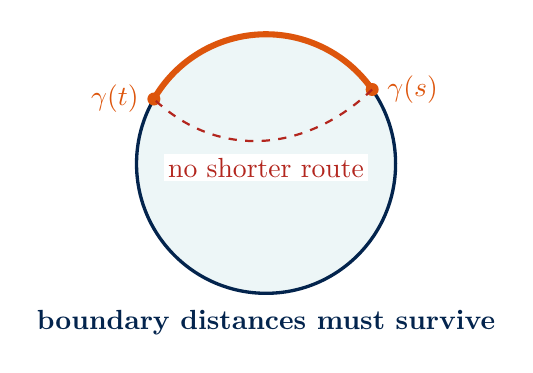
\begin{tikzpicture}[scale=0.94,>=Latex]
      \fill[DeepTeal!7] (0,0) circle (1.75);
      \draw[AuburnNavy,very thick] (0,0) circle (1.75);
      \coordinate (P) at (35:1.75);
      \coordinate (Q) at (150:1.75);
      \fill[AuburnOrange] (P) circle (2.5pt) node[right=2pt] {$\gamma(s)$};
      \fill[AuburnOrange] (Q) circle (2.5pt) node[left=2pt] {$\gamma(t)$};
      \draw[AuburnOrange,line width=2.2pt] (P)
      arc[start angle=35,end angle=150,radius=1.75];
      \draw[SoftRed,dashed,thick] (P) .. controls (0.55,0.15) and (-0.65,0.05) .. (Q);
      \node[SoftRed,fill=white,inner sep=1.5pt] at (0,-0.05) {no shorter route};
      \node[AuburnNavy,font=\bfseries] at (0,-2.15) {boundary distances must survive};
    \end{tikzpicture}
    \column{0.49\textwidth}
    \begin{block}{Isometric filling}
      A compact connected Riemannian surface $M$ with one boundary circle
      satisfies
      {\small\[
      d_M\bigl(\gamma(s),\gamma(t)\bigr)=d_{\T}(s,t)
      \qquad(s,t\in\T).
      \]}
    \end{block}
    \begin{itemize}
      \item Walking along the shorter boundary arc already gives ``$\le$''.
      \item The content is ``$\ge$'': the interior creates \alert{no shortcut}.
      \item The unit hemisphere honors the contract and has area $2\pi$.
    \end{itemize}
  \end{columns}
  \sourcefoot{Companion manuscript, Introduction, lines 115--148.}
  \note{Emphasize intrinsic distance: the surface may bend in ambient space, but only its internal metric matters. The red dashed path is forbidden from being shorter, not forbidden from existing.}
\end{frame}

\begin{frame}{Gromov's conjecture: the hemisphere should be cheapest}\label{fr:conjecture}
  \begin{block}{Filling-area conjecture (Gromov, 1983)}
    Every compact \alert{orientable} Riemannian isometric filling of the circle
    of circumference $2\pi$ should satisfy
    \[
      \boxed{\Area(M)\ge 2\pi},
    \]
    with equality for the unit round hemisphere.
  \end{block}
  \vspace{0.15cm}
  \begin{columns}[T,onlytextwidth]
    \column{0.32\textwidth}
    \statuspill{LeafGreen}{KNOWN}\quad disk case\par
    \small Gromov's theorem
    \column{0.32\textwidth}
    \statuspill{LeafGreen}{KNOWN}\quad genus one\par
    \small Bangert--Croke--Ivanov--Katz
    \column{0.32\textwidth}
    \statuspill{SoftRed}{OPEN}\quad general genus\par
    \small This is the conjecture
  \end{columns}
  \vspace{0.38cm}
  \begin{beamercolorbox}[rounded=true,sep=0.55em]{block body alerted}
    \centering\bfseries The theorem in this deck improves global lower bounds;
    it does not prove the conjectural value $2\pi$.
  \end{beamercolorbox}
  \sourcefoot{Gromov (1983); Bangert--Croke--Ivanov--Katz (2005); companion manuscript, lines 140--153.}
  \note{Pause on the status box. Students should leave knowing exactly what is theorem and what is conjecture.}
\end{frame}

\begin{frame}{A quantitative scoreboard}\label{fr:scoreboard}
  \begin{columns}[T,onlytextwidth]
    \column{0.60\textwidth}
    \small
    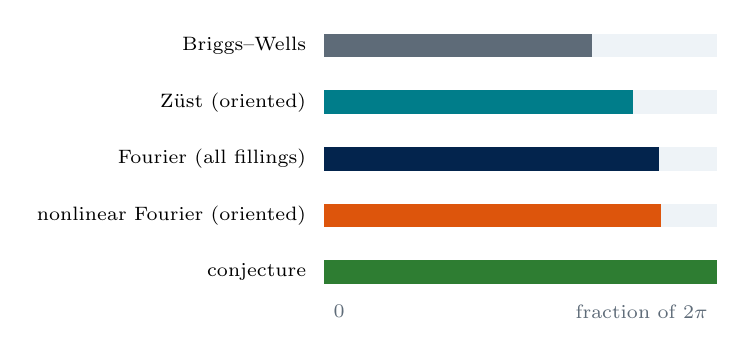
\begin{tikzpicture}[x=5.0cm,y=0.72cm]
      \foreach \y/\frac/\col/\lab in {
      4/0.68017/Slate/{Briggs--Wells},
      3/0.78539/DeepTeal/{Z\"ust (oriented)},
      2/0.85255/AuburnNavy/{Fourier (all fillings)},
      1/0.85781/AuburnOrange/{nonlinear Fourier (oriented)},
      0/1.00000/LeafGreen/{conjecture}}
      {
      \fill[Mist] (0,\y) rectangle (1,\y+0.42);
      \fill[\col] (0,\y) rectangle (\frac,\y+0.42);
      \node[anchor=east,font=\scriptsize] at (-0.02,\y+0.21) {\lab};
      }
      \node[anchor=west,font=\scriptsize,text=Slate] at (0,-0.48) {$0$};
      \node[anchor=east,font=\scriptsize,text=Slate] at (1,-0.48) {fraction of $2\pi$};
    \end{tikzpicture}
    \column{0.37\textwidth}
    \begin{tabular}{@{}l@{\ }r@{}}
      \toprule
      selected bound & value\\
      \midrule
      $\frac{\sqrt3}{4}\pi^2$ & $4.27366$\\
      $\frac{\pi^2}{2}$ & $4.93480$\\
      $\frac{14\zeta(3)}{\pi}$ & $5.35677$\\
      nonlinear & $>5.38982$\\
      \addlinespace
      conjecture & $6.28319$\\
      \bottomrule
    \end{tabular}
    \vspace{0.35cm}

    \small The last step is numerically modest but conceptually new: it is the
    first gain here that uses nonlinear relations among Fourier modes.
  \end{columns}
  \sourcefoot{Companion manuscript, lines 155--214. Values are rounded only on this overview frame.}
  \note{The plot shows selected bounds discussed in the manuscript, not a claim of a complete historical taxonomy. Point out the orientation hypotheses.}
\end{frame}

% =============================================================================
\section{The linear Fourier certificate}
% =============================================================================
\begin{frame}{The proof pipeline: one budget, many planar payoffs}\label{fr:pipeline}
  \centering
  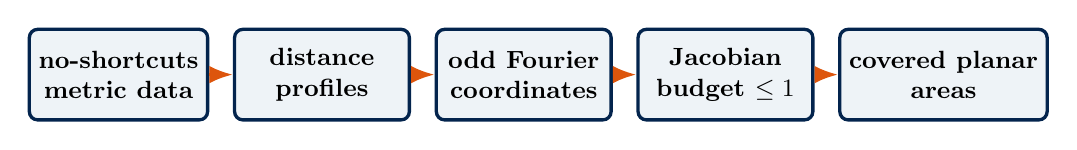
\begin{tikzpicture}[
    node distance=0.40cm and 0.30cm,
    box/.style={rounded corners=3pt,draw=AuburnNavy,very thick,fill=Mist,
    minimum width=2.22cm,minimum height=1.15cm,align=center,font=\small\bfseries},
    arr/.style={-{Latex[length=3mm]},very thick,AuburnOrange}]
    \node[box] (metric) {no-shortcuts\\metric data};
    \node[box,right=of metric] (profile) {distance\\profiles};
    \node[box,right=of profile] (fourier) {odd Fourier\\coordinates};
    \node[box,right=of fourier] (budget) {Jacobian\\budget $\le1$};
    \node[box,right=of budget] (payoff) {covered planar\\areas};
    \draw[arr] (metric)--(profile);
    \draw[arr] (profile)--(fourier);
    \draw[arr] (fourier)--(budget);
    \draw[arr] (budget)--(payoff);
  \end{tikzpicture}
  \vspace{0.55cm}
  \begin{columns}[T,onlytextwidth]
    \column{0.48\textwidth}
    \begin{exampleblock}{Analysis supplies the budget}
      Lipschitz functions + Rademacher + Bessel control how much total
      two-dimensional Jacobian the coordinates can spend.
    \end{exampleblock}
    \column{0.48\textwidth}
    \begin{alertblock}{Topology certifies the payoff}
      Boundary winding is converted into regions that every extension must
      cover, even when the filling is nonorientable.
    \end{alertblock}
  \end{columns}
  \sourcefoot{Companion manuscript, ``Structure of the argument,'' lines 216--257.}
  \note{This is the navigation frame. Revisit the five boxes verbally as each ingredient appears.}
\end{frame}

\begin{frame}{Distance profiles turn geometry into functions}\label{fr:profiles}
  \begin{columns}[T,onlytextwidth]
    \column{0.47\textwidth}
    \begin{block}{View the boundary from $x$}
      For every boundary label $\theta$,
      \[
        u_\theta(x)=d_M\bigl(x,\gamma(\theta)\bigr).
      \]
      Each $u_\theta$ is $1$-Lipschitz in $x$.
    \end{block}
    \small
    On the boundary, no shortcuts determine the whole profile:
    \[
      u_\theta(\gamma(s))=d_{\T}(s,\theta).
    \]
    The unknown interior geometry has acquired \alert{known boundary data}.
    \column{0.50\textwidth}
    \centering
    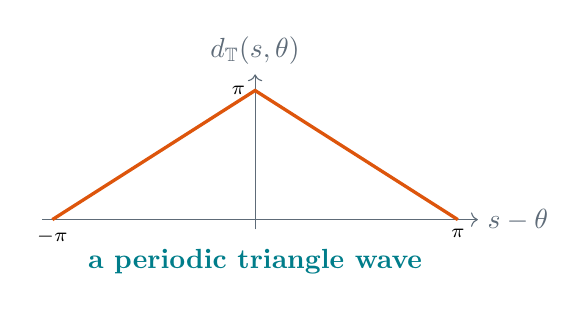
\begin{tikzpicture}[x=0.82cm,y=0.82cm]
      \draw[->,Slate] (-3.3,0)--(3.45,0) node[right] {$s-\theta$};
      \draw[->,Slate] (0,-0.15)--(0,2.25) node[above] {$d_{\T}(s,\theta)$};
      \draw[AuburnOrange,very thick]
      (-3.14,0)--(0,2)--(3.14,0);
      \node[below,font=\scriptsize] at (-3.14,0) {$-\pi$};
      \node[below,font=\scriptsize] at (3.14,0) {$\pi$};
      \node[left,font=\scriptsize] at (0,2) {$\pi$};
      \node[DeepTeal,font=\bfseries] at (0,-0.65) {a periodic triangle wave};
    \end{tikzpicture}
  \end{columns}
  \sourcefoot{Companion manuscript, Section 2, lines 259--314.}
  \note{This is the key modeling move. The surface is hard; a family of scalar 1-Lipschitz functions is familiar and Fourier-expandable.}
\end{frame}

\ifshowoddslack
\begin{frame}{Antipodes split the profile into signal and slack}\label{fr:odd-slack}
  \begin{columns}[T,onlytextwidth]
    \column{0.54\textwidth}
    \begin{align*}
      a_\theta(x)
      &=\frac{u_\theta(x)-u_{\theta+\pi}(x)}{2},
      &a_{\theta+\pi}&=-a_\theta,\\[0.4em]
      \sigma_\theta(x)
      &=\frac{u_\theta(x)+u_{\theta+\pi}(x)-\pi}{2},
      &\sigma_\theta&\ge0.
    \end{align*}
    \begin{block}{Almost-everywhere energy identity}
      \[
        \boxed{|\nabla a_\theta|^2+|\nabla\sigma_\theta|^2=1.}
      \]
    \end{block}
    \column{0.42\textwidth}
    \vspace{0.15cm}
    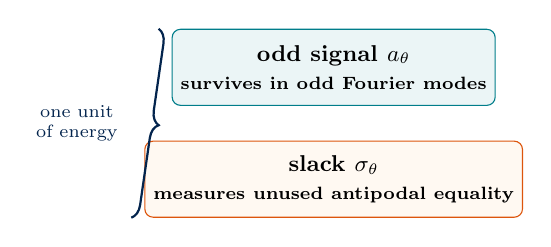
\begin{tikzpicture}[scale=0.92,transform shape,
      part/.style={rounded corners=3pt,minimum width=3.9cm,minimum height=1.05cm,
      align=center,font=\small\bfseries}]
      \node[part,draw=DeepTeal,fill=DeepTeal!8] (signal) {odd signal $a_\theta$\\\scriptsize survives in odd Fourier modes};
      \node[part,draw=AuburnOrange,fill=Cream,below=0.48cm of signal] (slack) {slack $\sigma_\theta$\\\scriptsize measures unused antipodal equality};
      \draw[decorate,decoration={brace,amplitude=5pt},AuburnNavy,thick]
      ([xshift=-0.18cm]signal.north west)--([xshift=-0.18cm]slack.south west)
      node[midway,left=7pt,align=center,font=\scriptsize] {one unit\\of energy};
    \end{tikzpicture}
    \vspace{0.28cm}

    \small On the boundary, $\sigma_\theta=0$: all boundary energy is signal.
  \end{columns}
  \sourcefoot{Companion manuscript, Definition 2.1 and equation (2.8), lines 279--393.}
  \note{First-year students can read this as a parallelogram identity. Stress that differentiability and the identity hold almost everywhere.}
\end{frame}
\fi

\begin{frame}{The Fourier camera sees exact boundary loops}\label{fr:fourier-camera}
  \begin{columns}[T,onlytextwidth]
    \column{0.50\textwidth}
    For odd $n\ge1$, define a planar coordinate
    \begin{align*}
      z_n(x)&=A_n(x)+iB_n(x),\\[-0.15em]
      z_n(x)&=\frac1\pi\int_0^{2\pi}
      a_\theta(x)e^{in\theta}\dd\theta.
    \end{align*}
    Anti-periodicity kills every even mode.

    \begin{alertblock}{Boundary miracle}
      \[
        \boxed{z_n(\gamma(s))=-\frac{4}{\pi n^2}e^{ins}.}
      \]
    \end{alertblock}
    \column{0.47\textwidth}
    \centering
    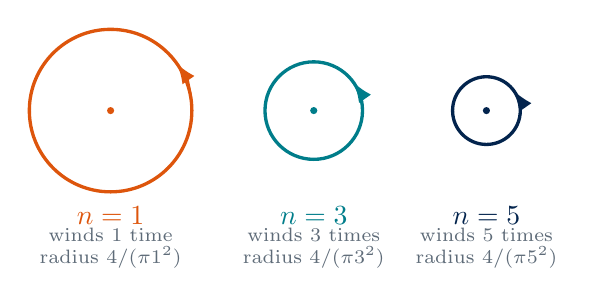
\begin{tikzpicture}[scale=0.86]
      \foreach \x/\n/\r/\col in {0/1/1.20/AuburnOrange,3.0/3/0.72/DeepTeal,5.55/5/0.50/AuburnNavy}{
      \draw[\col,very thick] (\x,0) circle (\r);
      \draw[-{Latex[length=2.5mm]},\col,thick] (\x+\r,0) arc[start angle=0,end angle=35,radius=\r];
      \fill[\col] (\x,0) circle (1.5pt);
      \node[font=\bfseries,\col] at (\x,-1.55) {$n=\n$};
      \node[font=\scriptsize,text=Slate,align=center] at (\x,-2.03) {winds $\n$ time\ifnum\n>1 s\fi\\radius $4/(\pi\n^2)$};
      }
    \end{tikzpicture}
  \end{columns}
  \sourcefoot{Companion manuscript, Sections 3--4, lines 394--434 and 486--523.}
  \note{The same unknown surface produces infinitely many planar maps, but their boundary loops are completely explicit. The radius decay is what makes the final series converge.}
\end{frame}

\begin{frame}{Bessel's inequality gives one shared Jacobian budget}\label{fr:budget}
  \begin{columns}[T,onlytextwidth]
    \column{0.56\textwidth}
    Select finitely many odd modes and mix them by any orthogonal matrix
    $U\in O(N)$:
    \[
      G_j=\sum_{k=1}^{N}u_{jk}F_{m_k},
      \qquad F_n=(A_n,B_n).
    \]
    At almost every point of $M$,
    \[
      \boxed{\sum_{j=1}^{N}J_2G_j\le1.}
    \]
    \small Orthogonal mixing redistributes the budget; it does not create new
    derivative energy.
    \column{0.40\textwidth}
    \centering
    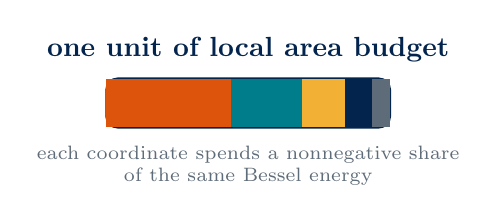
\begin{tikzpicture}[x=0.72cm,y=0.62cm]
      \draw[rounded corners=4pt,fill=Mist,draw=AuburnNavy,thick] (0,0) rectangle (5,1);
      \foreach \x/\w/\col in {0/2.2/AuburnOrange,2.2/1.25/DeepTeal,3.45/0.75/WarmGold,4.2/0.48/AuburnNavy,4.68/0.32/Slate}
      \fill[\col] (\x,0) rectangle +(\w,1);
      \node[above,font=\bfseries,AuburnNavy] at (2.5,1.15) {one unit of local area budget};
      \node[below,font=\scriptsize,text=Slate,align=center] at (2.5,-0.18)
      {each coordinate spends a nonnegative share\\of the same Bessel energy};
    \end{tikzpicture}
    \vspace{0.45cm}
    \begin{exampleblock}{Sharper version}
      The unused slack energy is subtracted from the right-hand side.
    \end{exampleblock}
  \end{columns}
  \sourcefoot{Companion manuscript, Proposition 3.2, lines 415--485.}
  \note{Do not derive the inequality here. The budget metaphor is the durable idea; the derivation is in backup.}
\end{frame}

\begin{frame}{Why nonorientability breaks the obvious winding argument}\label{fr:orientation}
  \begin{columns}[T,onlytextwidth]
    \column{0.47\textwidth}
    \begin{block}{On an oriented filling}
      A signed Jacobian and Stokes' theorem can read the integer winding of
      each boundary loop.
      \[
        \text{winding }n\quad\Longrightarrow\quad\text{signed area payoff}.
      \]
    \end{block}
    \centering
    \statuspill{LeafGreen}{SIGN CONSISTENT}
    \column{0.47\textwidth}
    \begin{alertblock}{On a nonorientable filling}
      A continuously chosen area sign does not exist. Local orientation can
      flip, so signed contributions cannot simply be added.
      \[
        n\text{-fold loop}\quad\not\Rightarrow\quad n\text{ signed sheets}.
      \]
    \end{alertblock}
    \centering
    \statuspill{SoftRed}{SIGN CAN FLIP}
  \end{columns}
  \vspace{0.50cm}
  \centering
  \Large\bfseries\color{AuburnNavy}
  Repair strategy: turn each multiple loop into a Jordan curve, then count
  coverage modulo $2$.
  \sourcefoot{Companion manuscript, Section 5, especially Lemmas 5.3--5.4.}
  \note{This is motivation, not a formal no-go theorem. The next two frames explain the actual repair.}
\end{frame}

\begin{frame}{Untwisting: orthogonal mixing makes every row simple}\label{fr:untwist}
  \begin{columns}[T,onlytextwidth]
    \column{0.44\textwidth}
    \small Start with boundary modes of frequencies
    \[
      1,3,5,\ldots,2N-1.
    \]
    An explicit product of Givens rotations produces $U_N\in O(N)$ whose
    every row satisfies
    \[
      \boxed{|u_{j1}|>
      \sum_{k=2}^{N}\frac{|u_{jk}|}{2k-1}.}
    \]
    The first harmonic outruns the combined derivative of all higher
    harmonics.
    \column{0.53\textwidth}
    \centering
    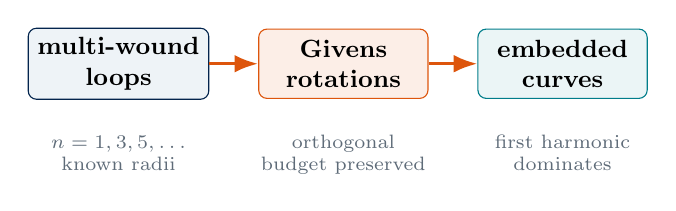
\begin{tikzpicture}[
      box/.style={rounded corners=3pt,draw=AuburnNavy,fill=Mist,
      minimum width=2.15cm,minimum height=0.88cm,align=center,font=\small\bfseries},
      arr/.style={-{Latex[length=3mm]},AuburnOrange,very thick}]
      \node[box] (loops) {multi-wound\\loops};
      \node[box,right=0.62cm of loops,fill=AuburnOrange!10,draw=AuburnOrange] (mix) {Givens\\rotations};
      \node[box,right=0.62cm of mix,fill=DeepTeal!8,draw=DeepTeal] (curves) {embedded\\curves};
      \draw[arr] (loops)--(mix);
      \draw[arr] (mix)--(curves);
      \node[below=0.33cm of loops,font=\scriptsize,text=Slate,align=center] {$n=1,3,5,\ldots$\\known radii};
      \node[below=0.33cm of mix,font=\scriptsize,text=Slate,align=center] {orthogonal\\budget preserved};
      \node[below=0.33cm of curves,font=\scriptsize,text=Slate,align=center] {first harmonic\\dominates};
    \end{tikzpicture}
    \vspace{0.52cm}
    \begin{exampleblock}{The design constraint}
      Change the boundary geometry without changing the total Jacobian budget.
    \end{exampleblock}
  \end{columns}
  \sourcefoot{Companion manuscript, Lemmas 5.1--5.2, lines 524--636.}
  \note{Givens rotations are the same two-coordinate rotations used in numerical linear algebra. Their role here is geometric: they redistribute the dominant frequency.}
\end{frame}

\begin{frame}{Jordan curves turn topology into guaranteed area}\label{fr:coverage}
  \begin{columns}[T,onlytextwidth]
    \column{0.47\textwidth}
    \centering
    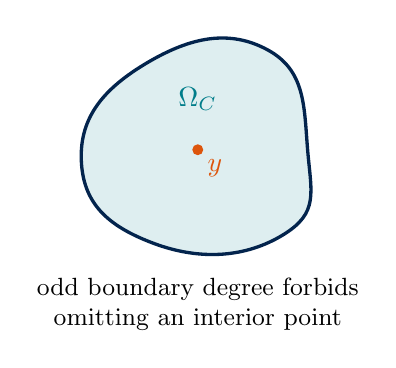
\begin{tikzpicture}[scale=0.90]
      \fill[DeepTeal!13]
      plot[smooth cycle,tension=0.85] coordinates
      {(0:1.55) (55:1.72) (120:1.42) (185:1.65) (245:1.46) (315:1.70)};
      \draw[AuburnNavy,very thick]
      plot[smooth cycle,tension=0.85] coordinates
      {(0:1.55) (55:1.72) (120:1.42) (185:1.65) (245:1.46) (315:1.70)};
      \fill[AuburnOrange] (0,0) circle (2.2pt) node[below right] {$y$};
      \node[DeepTeal,font=\bfseries] at (0,0.72) {$\Omega_C$};
      \node[align=center,font=\small] at (0,-2.18)
      {odd boundary degree forbids\\omitting an interior point};
    \end{tikzpicture}
    \column{0.50\textwidth}
    \begin{block}{Two facts do the work}
      \begin{enumerate}
        \item First-harmonic dominance makes $G_j|_{\partial M}$ a Jordan
        curve $C_j$ with explicit enclosed area.
        \item Mod-$2$ degree forces the bounded component
        $\Omega_{C_j}\subseteq G_j(M)$.
      \end{enumerate}
    \end{block}
    Hence the area formula gives
    \[
      \int_M J_2G_j\dd A\ge |\Omega_{C_j}|.
    \]
    \small No global orientation is needed: parity survives sign changes.
  \end{columns}
  \sourcefoot{Companion manuscript, Lemmas 5.3--5.4, lines 637--708.}
  \note{The contradiction is easy to state: if y were missed, radial projection around y would extend an odd-degree boundary map over M, impossible mod 2.}
\end{frame}

\begin{frame}{Add the payoffs, spend the budget once}\label{fr:universal}
  \begin{columns}[T,onlytextwidth]
    \column{0.58\textwidth}
    \begin{align*}
      \Area(M)
      &\ge \sum_{j=1}^{N}\int_M J_2G_j\dd A
      &&\text{(one shared budget)}\\
      &\ge \sum_{j=1}^{N}|\Omega_j|
      &&\text{(forced coverage)}\\
      &=\frac{16}{\pi}\sum_{k=1}^{N}\frac{1}{(2k-1)^3}
      &&\text{(orthogonality).}
    \end{align*}
    Let $N\to\infty$ and use
    \[
      \sum_{k\ge1}\frac1{(2k-1)^3}=\frac78\zeta(3).
    \]
    \column{0.38\textwidth}
    \bigconstant{$\displaystyle\Area(M)\ge\frac{14\zeta(3)}{\pi}$}{%
    $=5.3567723444\ldots$\\orientation-free}
    \vspace{0.38cm}
    \centering
    \statuspill{LeafGreen}{THEOREM}\par
    \vspace{0.2cm}
    \small\color{Slate}The conjectural target is still $2\pi$.
  \end{columns}
  \sourcefoot{Companion manuscript, Proposition 5.5 and Theorem 1.1, lines 709--748; exact Lean interface in \texttt{FORMALIZATION.md}.}
  \note{This is the linear climax. Walk down the three inequalities and identify which earlier frame paid for each one.}
\end{frame}

\ifshowoddslack
\begin{frame}{The discarded slack becomes an area defect}\label{fr:defect}
  \begin{block}{Antipodal defect refinement}
    Every isometric filling, orientable or not, satisfies
    \[
      \Area(M)\ge\frac{14\zeta(3)}{\pi}
      +\frac1{2\pi}\int_M\int_0^{2\pi}
      |\nabla\sigma_\theta(x)|^2\dd\theta\dd A(x).
    \]
  \end{block}
  \begin{columns}[T,onlytextwidth]
    \column{0.48\textwidth}
    \begin{exampleblock}{If slack varies}
      The baseline improves automatically by a nonnegative Dirichlet energy.
    \end{exampleblock}
    \column{0.48\textwidth}
    \begin{alertblock}{If the defect vanishes}
      The profile lies infinitesimally in the antipodal geometry of the
      injective hull; a different idea is needed.
    \end{alertblock}
  \end{columns}
  \vspace{0.35cm}
  \centering\large\bfseries\color{AuburnNavy}
  A good estimate is also a diagnostic: it tells us where improvement must hide.
  \sourcefoot{Companion manuscript, Theorem 6.1, lines 749--793.}
  \note{The defect is conceptually useful even if one does not use it numerically: either it pays area, or it forces a rigid profile geometry.}
\end{frame}
\fi

% =============================================================================
\section{The nonlinear gain}
% =============================================================================
\ifshowcalibration
\begin{frame}{Oriented area can be read by a calibration}\label{fr:calibration}
  \begin{columns}[T,onlytextwidth]
    \column{0.53\textwidth}
    Gather all odd coefficients into
    \[
      \mathcal H=\ell^2(1,3,5,\ldots;\C),
      \qquad Z:M\longrightarrow\mathcal H,
    \]
    \[
      Z(x)=(z_1(x),z_3(x),z_5(x),\ldots).
    \]
    The standard symplectic form
    \[
      \omega(p,q)=\sum_{n\ \mathrm{odd}>0}
      \operatorname{Im}(\overline{p_n}q_n)
    \]
    has comass at most $1$ on admissible tangent planes.
    \column{0.43\textwidth}
    \begin{block}{Area detector}
      \begin{align*}
        \int_{\partial M}Z^*\alpha
        &=\int_M Z^*\omega &&\text{(Stokes)}\\
        &\le \Area(M) &&\text{(comass $\le1$).}
      \end{align*}
      The left side is known from the boundary loop.
    \end{block}
    \small The boundary action equals $14\zeta(3)/\pi$, recovering the linear
    bound in the oriented setting.
  \end{columns}
  \sourcefoot{Companion manuscript, Section 7; exact status boundary in the slide claim ledger.}
  \note{Translate “comass” as the largest area density that the two-form can read on a unit tangent plane. The whole strategy is action divided by comass.}
\end{frame}
\fi

\ifshowbarriers
\begin{frame}{Two natural nonlinear ideas hit the same wall}\label{fr:barriers}
  \begin{columns}[T,onlytextwidth]
    \column{0.48\textwidth}
    \begin{alertblock}{Scalar feature engineering}
      Replacing each distance by a separate $1$-Lipschitz feature
      $\psi(u_\theta)$ cannot improve
      \[
        \frac{14\zeta(3)}{\pi}.
      \]
      A positive logarithmic kernel makes the original choice extremal.
    \end{alertblock}
    \column{0.48\textwidth}
    \begin{alertblock}{Ambient Hilbert geometry}
      The boundary Fourier loop spans a holomorphic disk whose Euclidean area
      is already
      \[
        \frac{14\zeta(3)}{\pi}.
      \]
      No Euclidean-comass-$1$ form can read more action.
    \end{alertblock}
  \end{columns}
  \vspace{0.42cm}
  \begin{beamercolorbox}[rounded=true,sep=0.55em,center]{block body example}
    \bfseries To gain, couple modes genuinely nonlinearly and exploit the
    smaller $L^\infty$ geometry of actual distance profiles.
  \end{beamercolorbox}
  \sourcefoot{Companion manuscript, Propositions 8.1--8.2, lines 905--1032. Each barrier is limited to its stated class.}
  \note{These are productive failures: they identify exactly which geometry the successful perturbation must use.}
\end{frame}
\fi

\begin{frame}{Phase resonance: a cubic term lands on the right frequency}\label{fr:resonance}
  \begin{columns}[T,onlytextwidth]
    \column{0.55\textwidth}
    For $n=1,3,5,\ldots$, perturb the coordinate by
    \[
      (\mathcal G_\lambda(z))_n
      =z_n+\lambda\,\overline{z_1}^{,2}z_{n+2}.
    \]
    On the boundary,
    \[
      \overline{e^{is}}^{,2}e^{i(n+2)s}=e^{ins}.
    \]
    The cubic correction has \alert{exactly the same phase} as $z_n$.
    \column{0.41\textwidth}
    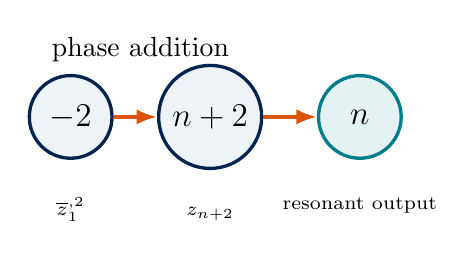
\begin{tikzpicture}[
      token/.style={circle,minimum size=1.05cm,draw=AuburnNavy,very thick,
      fill=Mist,font=\large\bfseries},
      arr/.style={-{Latex[length=2.6mm]},AuburnOrange,very thick}]
      \node[token] (m2) {$-2$};
      \node[token,right=0.55cm of m2] (np2) {$n+2$};
      \node[token,right=0.68cm of np2,fill=DeepTeal!10,draw=DeepTeal] (n) {$n$};
      \node at ($(m2)!0.5!(np2)+(0,0.86)$) {phase addition};
      \draw[arr] (m2)--(np2);
      \draw[arr] (np2)--(n);
      \node[below=0.35cm of m2,font=\scriptsize,align=center] {$\overline z_1^{,2}$};
      \node[below=0.35cm of np2,font=\scriptsize] {$z_{n+2}$};
      \node[below=0.35cm of n,font=\scriptsize] {resonant output};
    \end{tikzpicture}\par
    \vspace{0.55cm}
    \begin{exampleblock}{Boundary payoff}
      $\mathcal B(\lambda)=C_0+b\lambda+d\lambda^2$ with $b>0$.
    \end{exampleblock}
  \end{columns}
  \sourcefoot{Companion manuscript, Sections 9--10, lines 1033--1141.}
  \note{This is just frequency arithmetic: conjugating z1 twice contributes frequency minus two, which cancels the shift from n+2 back to n.}
\end{frame}

\begin{frame}{The key asymmetry: gain is linear, cost is quadratic}\label{fr:stationarity}
  \begin{columns}[T,onlytextwidth]
    \column{0.53\textwidth}
    At a plane saturating the linear comass, the boundary-direction field is
    analytic or anti-analytic with $|W|=1$. Therefore its nonzero
    autocorrelation vanishes:
    \[
      \sum_{\substack{n>0\\ n\,\mathrm{odd}}}
      c_n\overline{c_{n+2}}=0.
    \]
    This kills the first variation of the comass.
    \[
      \boxed{\begin{aligned}
        \text{boundary gain}&=O(\lambda),\\
        \text{comass cost}&=O(\lambda^2).
      \end{aligned}}
    \]
    \column{0.43\textwidth}
    \centering
    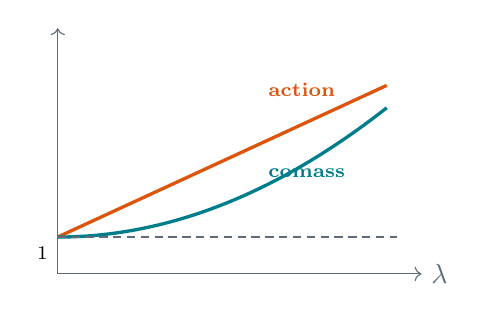
\begin{tikzpicture}[x=4.4cm,y=2.6cm]
      \draw[->,Slate] (0,0)--(1.05,0) node[right] {$\lambda$};
      \draw[->,Slate] (0,0)--(0,1.20);
      \draw[AuburnOrange,very thick] plot[domain=0:0.95,samples=40] (\x,{0.18+0.78*\x});
      \draw[DeepTeal,very thick] plot[domain=0:0.95,samples=40] (\x,{0.18+0.70*\x*\x});
      \node[AuburnOrange,anchor=west,font=\scriptsize\bfseries] at (0.58,0.90) {action};
      \node[DeepTeal,anchor=west,font=\scriptsize\bfseries] at (0.58,0.49) {comass};
      \draw[densely dashed,Slate] (0,0.18)--(0.98,0.18);
      \node[below left,font=\scriptsize] at (0,0.18) {$1$};
    \end{tikzpicture}\par
    \vspace{0.28cm}
    \small\color{Slate}The picture is schematic; the theorem uses explicit global constants.
  \end{columns}
  \sourcefoot{Companion manuscript, Sections 10--11; exact status boundary in the slide claim ledger.}
  \note{This is the conceptual heart. A perturbation can improve a quotient when its numerator has positive slope and its denominator is stationary.}
\end{frame}

\begin{frame}{An explicit nonlinear certificate}\label{fr:nonlinear}
  \begin{columns}[T,onlytextwidth]
    \column{0.57\textwidth}
    For $0\le\lambda<\pi^2/32$,
    \[
      \Area(M)\ge
      \frac{\mathcal B(\lambda)}{\mathcal C(\lambda)}
      =\frac{C_0+b\lambda+d\lambda^2}
      {1+\lambda^2\left[Q_*+
      \dfrac{C_*^2}{4(1-D_*\lambda)}\right]}.
    \]
    At $\lambda=0.03$,
    \[
      \mathcal B=5.4230028938\ldots,
      \qquad
      \mathcal C=1.0061557533\ldots.
    \]
    \column{0.39\textwidth}
    \bigconstant{$\displaystyle\Area(M)>5.38982446$}{%
    every compact connected oriented\\Riemannian isometric filling}
    \vspace{0.40cm}
    \centering\statuspill{LeafGreen}{THEOREM}\par
    \vspace{0.20cm}
    \small\color{Slate}Numerical optimum of this estimate: $5.38984897\ldots$.
  \end{columns}
  \sourcefoot{Companion manuscript, Theorem 12.1 and its evaluation, lines 1510--1581; exact Lean interface in \texttt{FORMALIZATION.md}.}
  \note{The strict decimal endpoint is chosen below the evaluated ratio and is formally verified. The optimized decimal is explanatory, not the displayed certified theorem endpoint.}
\end{frame}

\ifshowfrontier
\begin{frame}{The method has a ceiling---and the problem has new routes}\label{fr:frontier}
  \begin{columns}[T,onlytextwidth]
    \column{0.42\textwidth}
    \begin{alertblock}{A precise limitation}
      The normalized \emph{one-high-leg} resonance hierarchy, when certified by
      a global ambient comass bound, satisfies
      \[
        \text{certificate}<5.466.
      \]
    \end{alertblock}
    \small This is not a ceiling for every nonlinear Fourier method.
    \column{0.54\textwidth}
    \begin{exampleblock}{Three routes beyond it}
      \begin{enumerate}
        \item a Fourier--Z\"ust profile-adapted hybrid;
        \item a de Sitter comparison inequality for profile geometry;
        \item genuinely multi-high-leg, low-mode corrections.
      \end{enumerate}
    \end{exampleblock}
    \begin{block}{The remaining numerical gap}
      \[
        2\pi-5.38982446\approx0.89336.
      \]
    \end{block}
  \end{columns}
  \sourcefoot{Companion manuscript, Sections 13--16 and 18, especially lines 1582--1988 and 2616--2676.}
  \note{Treat a negative result as navigation. The ceiling rules out repeatedly adding the same kind of phase correction; it points toward profile-adapted geometry.}
\end{frame}
\fi

% =============================================================================
\section{Claim boundary}
% =============================================================================
\ifshowverification
\begin{frame}{What is verified, what is not}\label{fr:verified-boundary}
  \small
  \begin{tabular}{@{}p{0.18\textwidth}p{0.74\textwidth}@{}}
    \toprule
    \good & Both headline surface-area bounds at their explicit Riemannian
    interfaces; the Fourier algebra, topological coverage, area certificates,
    and rigorous endpoint numerics used in those closures.\\[0.45em]
    \partialstatus & Several broader standalone manuscript formulations,
    including general Hilbert-valued Stokes/comass statements and later
    resonance/operator bridges.\\[0.45em]
    \openstatus & Gromov's sharp $2\pi$ conjecture, the full nonlinear frontier,
    and any definitive priority judgment.\\
    \bottomrule
  \end{tabular}
  \vspace{0.38cm}
  \begin{beamercolorbox}[rounded=true,sep=0.55em]{block body alerted}
    \centering\bfseries Kernel verification checks exact formal statements; it
    does not turn a stronger nearby sentence into a theorem.
  \end{beamercolorbox}
  \vspace{0.30cm}
  \centering
  \statuspill{LeafGreen}{6,677 PROJECT DECLARATIONS AUDITED}\quad
  \statuspill{LeafGreen}{NO PROJECT PROOF ESCAPES}
  \sourcefoot{Repository \texttt{FORMALIZATION.md}, complete 27-item ledger and trust-evidence section at commit \texttt{f166e04}.}
  \note{This frame is part of the mathematical content: it prevents verified components, verified headline closures, and open neighboring claims from being conflated.}
\end{frame}
\fi

\begin{frame}[plain,noframenumbering]\label{fr:takeaways}
  \begin{tikzpicture}[remember picture,overlay]
    \fill[AuburnNavy] (current page.south west) rectangle (current page.north east);
    \fill[AuburnOrange] (current page.south west) rectangle
    ([xshift=0.20cm]current page.north west);
  \end{tikzpicture}
  \color{white}
  {\LARGE\bfseries Three ideas to take home}\par
  \vspace{0.48cm}
  \begin{enumerate}
    \setlength{\itemsep}{0.50em}
    \item \textcolor{white}{The no-shortcuts condition converts an unknown surface
    into distance profiles with exact boundary data.}
    \item \textcolor{white}{Fourier modes share one Jacobian budget; topology turns
    their boundary curves into planar area certificates.}
    \item \textcolor{white}{Nonlinear phase resonance gains because boundary action
    moves at first order while the comass is stationary.}
  \end{enumerate}
  \vfill
  \begin{center}
  {\Large\color{WarmGold}\bfseries The best bound here is $5.38982446$; the
  conjectural $2\pi$ remains open.}\par
  \vspace{0.42cm}
  {\large Questions?}
  \end{center}
  \note{End on the open conjecture, not on the formalization machinery. Invite questions using the technical backup frames.}
\end{frame}

% =============================================================================
% BACKUP / MOTHER-DECK MODULES
% =============================================================================
\appendix
\section{Technical backup}

\begin{frame}{Backup: the metric contract in one line}\label{bk:metric}
  Let $\T=\R/2\pi\mathbb Z$ with
  \[
    d_{\T}(s,t)=\min_{k\in\mathbb Z}|s-t+2\pi k|.
  \]
  If $\gamma:\T\to\partial M$ is arclength parametrized, traveling on the
  boundary gives
  \[
    d_M(\gamma(s),\gamma(t))\le d_{\T}(s,t).
  \]
  Thus ``isometric filling'' is exactly the reverse inequality:
  \[
    \boxed{d_M(\gamma(s),\gamma(t))\ge d_{\T}(s,t).}
  \]
  \begin{exampleblock}{Scaling}
    Circumference $2\pi$ is a normalization. For boundary length $\ell$, all
    area bounds scale by $(\ell/2\pi)^2$.
  \end{exampleblock}
  \sourcefoot{Companion manuscript, Introduction and Section 19.}
\end{frame}

\begin{frame}{Backup: the triangle-wave coefficient}\label{bk:triangle}
  On $[-\pi,\pi]$, the centered boundary profile is
  $q(t)=|t|-\pi/2$. For $n\ge1$,
  \[
    \frac1\pi\int_{-\pi}^{\pi}|t|\cos(nt)\dd t
    =\frac{2}{\pi n^2}\bigl((-1)^n-1\bigr).
  \]
  Therefore
  \[
    \widehat q(n)=
    \begin{cases}
      -4/(\pi n^2),&n\text{ odd},\\
      0,&n\text{ even}.
    \end{cases}
  \]
  Translating the triangle wave by $s$ contributes the phase $e^{ins}$, giving
  $z_n(\gamma(s))=-(4/(\pi n^2))e^{ins}$.
  \sourcefoot{Companion manuscript, Lemma 4.1.}
\end{frame}

\begin{frame}{Backup: from Bessel energy to a Jacobian budget}\label{bk:budget-proof}
  At a regular point choose an orthonormal basis $(e_1,e_2)$ and write
  \[
    f(\theta)=\dd a_\theta(e_1),\qquad
    g(\theta)=\dd a_\theta(e_2).
  \]
  Bessel's inequality for the selected Fourier modes and orthogonality of $U$
  give
  \[
    \sum_j\bigl(|\dd G_j(e_1)|^2+|\dd G_j(e_2)|^2\bigr)
    \le\frac1\pi\int_0^{2\pi}(f^2+g^2)\dd\theta.
  \]
  Since $J_2L\le\tfrac12(|L e_1|^2+|L e_2|^2)$,
  \[
    \sum_jJ_2G_j
    \le\frac1{2\pi}\int|\nabla a_\theta|^2\dd\theta
    =1-\frac1{2\pi}\int|\nabla\sigma_\theta|^2\dd\theta.
  \]
  \sourcefoot{Companion manuscript, Proposition 3.2.}
\end{frame}

\begin{frame}{Backup: the Givens rotations are explicit}\label{bk:givens}
  For $m_k=2k-1$ and $w_k=1/m_k$, set
  \[
    c_k=(1+4w_k^2)^{-1/2},\qquad
    s_k=2w_k(1+4w_k^2)^{-1/2}.
  \]
  Let $R_k$ rotate only the $(1,k)$ coordinate plane by
  \[
    \begin{pmatrix}c_k&-s_k\\s_k&c_k\end{pmatrix},
    \qquad U_N=R_2R_3\cdots R_N.
  \]
  The estimates
  \[
    c_k\ge e^{-2w_k^2},\qquad
    \sum_{k\ge2}\frac1{(2k-1)^2}<\frac14
  \]
  yield the rowwise first-harmonic dominance required in the main talk.
  \sourcefoot{Companion manuscript, Lemmas 5.1--5.2.}
\end{frame}

\begin{frame}{Backup: why first-harmonic dominance gives a Jordan curve}\label{bk:jordan}
  Suppose
  \[
    z(s)=\sum_{k=1}^{N}a_ke^{im_ks},
    \qquad
    |a_1|>\sum_{k=2}^{N}m_k|a_k|.
  \]
  Since $|e^{ims}-e^{imt}|\le m|e^{is}-e^{it}|$,
  \[
    |z(s)-z(t)|\ge
    \left(|a_1|-\sum_{k\ge2}m_k|a_k|\right)|e^{is}-e^{it}|>0.
  \]
  Hence $z$ is embedded. Straight-line homotopy to $a_1e^{is}$ avoids the
  origin, so its winding is $+1$, and Green's formula gives
  \[
    |\Omega_z|=\pi\sum_{k=1}^{N}m_k|a_k|^2.
  \]
  \sourcefoot{Companion manuscript, Lemma 5.3.}
\end{frame}

\begin{frame}{Backup: the mod-$2$ coverage contradiction}\label{bk:mod2}
  Let $G:M\to\R^2$ be continuous and suppose $G|_{\partial M}$ is a Jordan
  curve $C$. If $y\in\Omega_C$ were omitted by $G(M)$, radial projection about
  $y$ would produce
  \[
    r_y\circ G:M\longrightarrow S^1.
  \]
  Its boundary restriction has odd degree because $y$ lies inside $C$.

  But over $\mathbb Z_2$, the boundary class of a compact surface is the
  boundary of the relative fundamental class:
  \[
    [\partial M]=\partial[M,\partial M]_2.
  \]
  It must therefore map to zero in $H_1(S^1;\mathbb Z_2)$---a contradiction.
  Thus $\Omega_C\subseteq G(M)$.
  \sourcefoot{Companion manuscript, Lemma 5.4.}
\end{frame}

\begin{frame}{Backup: the finite certificate telescopes conceptually}\label{bk:finite-certificate}
  With $\rho_m=4/(\pi m^2)$, the $j$th mixed boundary curve encloses
  \[
    |\Omega_j|=\pi\sum_{k=1}^{N}m_k\rho_{m_k}^2u_{jk}^2.
  \]
  Sum in $j$ and use the column identity $\sum_j u_{jk}^2=1$:
  \begin{align*}
    \sum_j|\Omega_j|
    &=\pi\sum_km_k\rho_{m_k}^2\sum_ju_{jk}^2\\
    &=\frac{16}{\pi}\sum_{k=1}^{N}\frac1{m_k^3}.
  \end{align*}
  The topology supplies each $|\Omega_j|$; orthogonality makes all dependence
  on the mixing matrix disappear after summation.
  \sourcefoot{Companion manuscript, Proposition 5.5.}
\end{frame}

\begin{frame}{Backup: calibration and comass vocabulary}\label{bk:comass}
  For a two-form $\omega$, its comass on the admissible unit tangent planes is
  \[
    \|\omega\|_{\mathrm{comass}}
    =\sup_{(e_1,e_2)}|\omega(e_1,e_2)|.
  \]
  If $\omega=\dd\alpha$, Stokes and the area bound give
  \[
    \left|\int_{\partial M}G^*\alpha\right|
    =\left|\int_MG^*\omega\right|
    \le\|\omega\|_{\mathrm{comass}}\Area(M).
  \]
  Therefore every such construction yields the certificate
  \[
    \boxed{\Area(M)\ge
    \frac{\text{boundary action}}{\text{global comass bound}}.}
  \]
  The nonlinear problem is an optimization of this quotient.
  \sourcefoot{Companion manuscript, Sections 7 and 12.}
\end{frame}

\begin{frame}{Backup: exact boundary action of the resonance}\label{bk:boundary-action}
  The perturbed boundary radius is
  \[
    \rho_n+\lambda\rho_1^2\rho_{n+2},
    \qquad \rho_n=\frac4{\pi n^2}.
  \]
  Hence
  \[
    \mathcal B(\lambda)
    =\pi\sum_{\substack{n>0\\ n\,\mathrm{odd}}}
    n\bigl(\rho_n+\lambda\rho_1^2\rho_{n+2}\bigr)^2
    =C_0+b\lambda+d\lambda^2,
  \]
  where
  \[
    C_0=\frac{14\zeta(3)}\pi,
    \quad
    b=\frac{512}{\pi^3}\left(\frac34-\frac{\pi^2}{16}\right)>0,
  \]
  \[
    d=\frac{4096}{\pi^5}
    \left(\frac78\zeta(3)+1-\frac{\pi^4}{48}\right)>0.
  \]
  \sourcefoot{Companion manuscript, Proposition 9.1.}
\end{frame}

\begin{frame}{Backup: quantitative comass control}\label{bk:comass-bound}
  If $\delta=1-|\Omega_0|$ measures the deficit from linear saturation, the
  first and second variations obey
  \[
    |L|\le C_*\sqrt\delta+D_*\delta,
    \qquad |Q|\le Q_*.
  \]
  Optimizing over $\delta\in[0,1]$ gives, for $0\le\lambda<\pi^2/32$,
  \[
    \|\Omega_\lambda\|_{\mathrm{comass}}
    \le1+\lambda^2\left[
    Q_*+\frac{C_*^2}{4(1-D_*\lambda)}
    \right].
  \]
  Here
  \[
    C_*=\frac{8\sqrt2}{3},\quad
    D_*=\frac{32}{\pi^2},\quad
    Q_*=\frac{128}{9\pi^2}+\frac{1280}{9\pi^4}.
  \]
  \sourcefoot{Companion manuscript, Proposition 11.1.}
\end{frame}

\begin{frame}{Backup: certified arithmetic at $\lambda=0.03$}\label{bk:lambda}
  The one-parameter certificate evaluates to
  \[
    \frac{\mathcal B(0.03)}{\mathcal C(0.03)}
    =\frac{5.4230028938\ldots}{1.0061557533\ldots}
    =5.3898244639\ldots.
  \]
  Thus the safely rounded theorem endpoint is
  \[
    \boxed{\Area(M)>5.38982446.}
  \]
  Numerically optimizing the explicit lower-bound formula gives
  \[
    \lambda\approx0.029227,
    \qquad \Area(M)\ge5.3898489672\ldots.
  \]
  \begin{alertblock}{Status distinction}
    The strict $5.38982446$ endpoint is the displayed verified theorem; the
    numerical optimum explains the formula but is not substituted for it.
  \end{alertblock}
  \sourcefoot{Companion manuscript, evaluation after Theorem 12.1; formalization ledger, Theorem 1.2 row.}
\end{frame}

\begin{frame}{Backup: the one-high-leg spectral ceiling}\label{bk:ceiling}
  For a normalized finite hierarchy, the unavoidable high-mode test gives
  \[
    \mathfrak C_J(\boldsymbol\mu)\ge1+\sum_{j=1}^{J}\mu_j^2.
  \]
  Meanwhile the boundary action is the quadratic form $x^TM^{(J)}x$, with
  \[
    M_{jk}=\frac{16}{\pi}
    \sum_{\substack{n>0\\ n\,\mathrm{odd}}}
    \frac{n}{(n+2j)^2(n+2k)^2}.
  \]
  Therefore every such certificate is bounded by
  $\lambda_{\max}(M^{(J)})$. The manuscript proves the infinite-operator bound
  \[
    \boxed{\|M\|<5.466.}
  \]
  \small The formalization ledger records the finite algebra and trace
  arithmetic as verified pieces, while the full operator/comass bridge remains
  partial or open.
  \sourcefoot{Companion manuscript, Section 14; \texttt{FORMALIZATION.md}, Theorem 14.2 through Theorem 14.4 rows.}
\end{frame}

\begin{frame}{Backup: rescaling to any circumference}\label{bk:scaling}
  If the boundary circumference is $\ell$, rescale lengths by $2\pi/\ell$.
  Areas scale quadratically, so the orientation-free theorem becomes
  \[
    \boxed{\Area(M)\ge
    \frac{7\zeta(3)}{2\pi^3}\,\ell^2.}
  \]
  The oriented nonlinear bound scales by the same factor:
  \[
    \Area(M)>
    5.38982446\left(\frac{\ell}{2\pi}\right)^2.
  \]
  The hemisphere benchmark becomes
  \[
    2\pi\left(\frac{\ell}{2\pi}\right)^2
    =\frac{\ell^2}{2\pi}.
  \]
  \sourcefoot{Companion manuscript, Section 19.}
\end{frame}

\section{Verification and references}
\begin{frame}{Backup: exact formalization boundary}\label{bk:formalization}
  \scriptsize
  \begin{tabular}{@{}p{0.24\textwidth}p{0.68\textwidth}@{}}
    \toprule
    Item & Repository status at \texttt{f166e04}\\
    \midrule
    Universal Fourier bound & \good{} at the exact compact connected
    Riemannian filling interface recorded in the ledger.\\
    Explicit nonlinear improvement & \good{} at the project-defined
    conventional orientation interface; strict decimal endpoint and
    all-parameter formula.\\
    Core ingredients & Fourier algebra, Givens mixing, degree/Jordan coverage,
    intrinsic area inequality, certificate logic, and rational numerics are
    verified in the headline closures.\\
    Broader formulations & General raw-distance eikonal, generic
    Hilbert-valued Stokes/comass, and several later resonance/operator items
    are partial or open as standalone manuscript claims.\\
    Trust receipt & GitHub Actions run \texttt{33504856733}; 6,677 project
    declarations audited; allowed axioms exactly \texttt{propext},
    \texttt{Classical.choice}, and \texttt{Quot.sound}.\\
    \bottomrule
  \end{tabular}\par
  \vspace{0.35cm}
  \centering\bfseries\color{AuburnOrange}
  No repository statement proves the conjectural $2\pi$ bound.
  \sourcefoot{Repository \texttt{FORMALIZATION.md}, frozen blob listed in the slide README.}
\end{frame}

\begin{frame}{References I: the conjecture and known cases}\label{bk:refs1}
  \footnotesize
  \textbf{M. Gromov} (1983), ``Filling Riemannian manifolds,''
  \emph{J. Differential Geometry} \textbf{18}, 1--147.\\[-0.15em]
  \href{https://doi.org/10.4310/jdg/1214509283}{\textbf{DOI}:10.4310/jdg/1214509283}
  \;|\;
  \href{https://mathscinet.ams.org/mathscinet-getitem?mr=697984}{MR697984}

  \vspace{0.62cm}
  \textbf{V. Bangert, C. Croke, S. Ivanov, and M. Katz} (2005),
  ``Filling area conjecture and ovalless real hyperelliptic surfaces,''
  \emph{Geom. Funct. Anal.} \textbf{15}, 577--597.\\[-0.15em]
  \href{https://doi.org/10.1007/s00039-005-0517-8}{\textbf{DOI}:10.1007/s00039-005-0517-8}
  \;|\;
  \href{https://mathscinet.ams.org/mathscinet-getitem?mr=2221144}{MR2221144}
  \;|\;
  \href{https://arxiv.org/abs/math/0405583}{arXiv:math/0405583}

  \vspace{0.65cm}
  \begin{beamercolorbox}[rounded=true,sep=0.5em]{block body example}
    These primary sources support the conjecture statement and the disk/genus-one
    status summary used in the core deck.
  \end{beamercolorbox}
\end{frame}

\begin{frame}{References II: recent bounds}\label{bk:refs2}
  \scriptsize
  \textbf{R. Z\"ust} (2025), ``The Riemannian hemisphere is almost calibrated
  in the injective hull of its boundary,'' \emph{Calc. Var. PDE} \textbf{64},
  Art. 297.\\[-0.15em]
  \href{https://doi.org/10.1007/s00526-025-03133-z}{\textbf{DOI}:10.1007/s00526-025-03133-z}
  \;|\;
  \href{https://arxiv.org/abs/2104.04498}{arXiv:2104.04498}

  \vspace{0.42cm}
  \textbf{J. Briggs and C. Wells} (2026), ``A discrete view of Gromov's filling
  area conjecture.''\\[-0.15em]
  \href{https://arxiv.org/abs/2602.17859}{arXiv:2602.17859}

  \vspace{0.42cm}
  \textbf{L. Chen, X. Li, and Y. Zhong} (2026), ``Fourier and resonant nonlinear
  bounds for Gromov's filling area problem,'' companion manuscript.\\[-0.15em]
  \href{https://github.com/lowrank/conj-gromov-filling/blob/f166e04054b397efdcb7c1ac5217ede715c1cfd0/fourier_resonant_filling_area_v3.tex}{private source snapshot}
  \;|\;
  \href{https://github.com/lowrank/conj-gromov-filling/blob/f166e04054b397efdcb7c1ac5217ede715c1cfd0/FORMALIZATION.md}{formalization ledger}

  \vspace{0.52cm}
  \begin{beamercolorbox}[rounded=true,sep=0.48em]{block body alerted}
    \centering The repository is private. These last two links require
    collaborator access and are not an authorization to redistribute the source.
  \end{beamercolorbox}
\end{frame}

\end{document}
